%==========================================================================
% ARTIGO CIENTÍFICO — EIC
% Automatic Detection and Classification of Buds in Grapevines
% Using Computer Vision and Deep Learning
%==========================================================================
\documentclass[12pt, a4paper]{article}

% --- Codificação e Língua ---
\usepackage[utf8]{inputenc}
\usepackage[T1]{fontenc}
\usepackage[english,portuguese]{babel}

% --- Layout ---
\usepackage[top=2.5cm, bottom=2.5cm, left=2.5cm, right=2.5cm]{geometry}
\usepackage{setspace}
\onehalfspacing

% --- Fontes ---
\usepackage{lmodern}
\usepackage{microtype}

% --- Gráficos ---
\usepackage{graphicx}
\usepackage{float}
\usepackage{caption}
\usepackage{subcaption}
\usepackage[table,xcdraw]{xcolor}

% --- Tabelas ---
\usepackage{booktabs}
\usepackage{tabularx}
\usepackage{multirow}

% --- Matemática ---
\usepackage{amsmath}
\usepackage{amssymb}

% --- Listas ---
\usepackage{enumitem}

% --- Código ---
\usepackage{listings}
\lstset{basicstyle=\ttfamily\small, breaklines=true, frame=single,
        numbers=left, numberstyle=\tiny, captionpos=b}

% --- Hiperlinks ---
\usepackage[colorlinks=true, linkcolor=blue!60!black,
            citecolor=green!50!black, urlcolor=blue!70!black,
            pdftitle={Automatic Detection and Classification of Buds in
                      Grapevines Using Computer Vision and Deep Learning},
            pdfauthor={Robson Alexander Alves}]{hyperref}

% --- Referências ---
\usepackage[backend=biber, style=numeric, sorting=nyt]{biblatex}
\addbibresource{referencias.bib}

% --- Outros ---
\usepackage{csquotes}
\usepackage{abstract}
\usepackage{titlesec}

% Formatação das secções
\titleformat{\section}{\large\bfseries}{\thesection.}{0.5em}{}
\titleformat{\subsection}{\normalsize\bfseries}{\thesubsection.}{0.5em}{}

%==========================================================================
\begin{document}
%==========================================================================

%--------------------------------------------------------------------------
% CABEÇALHO
%--------------------------------------------------------------------------
\begin{center}
  {\LARGE \textbf{Deteção e Classificação Automática de Gomos em Videiras
  utilizando Visão Computacional e \textit{Deep Learning}}}

  \vspace{0.8em}

  {\large Robson Alexander Alves$^{1}$, Inês Sena$^{1}$,
          João Mendes$^{1}$, Maurício Morais$^{1}$}

  \vspace{0.4em}

  {\small $^{1}$Research Centre in Digitalization and Intelligent Robotics
  (CeDRI), Laboratório para a Sustentabilidade e Tecnologia em Regiões de
  Montanha (SusTEC), Instituto Politécnico de Bragança, Campus de Santa
  Apolónia, 5300-253 Bragança, Portugal}

  \vspace{0.2em}

  {\small \texttt{a67712@alunos.ipb.pt} $\cdot$
          \texttt{ines.sena@ipb.pt} $\cdot$
          \texttt{joao.cmendes@ipb.pt} $\cdot$
          \texttt{mauricio@ipb.pt}}
\end{center}

\vspace{1em}
\noindent\rule{\textwidth}{0.4pt}

%--------------------------------------------------------------------------
% RESUMO
%--------------------------------------------------------------------------
\begin{abstract}
\noindent
A poda mecanizada da videira requer a identificação precisa dos gomos,
estruturas de pequena dimensão que determinam os pontos de corte. Este
artigo descreve o desenvolvimento de um sistema de deteção automática de
gomos em videiras, baseado no modelo \textit{YOLO26 Nano} e treinado sobre
dois datasets distintos na plataforma Roboflow. Foram desenvolvidos três modelos incrementais: o primeiro utilizou o
dataset público \textit{Segmentation-Vineyard-2}, de origem espanhola,
ao qual foram adicionadas manualmente anotações da classe \textit{gomo},
ausente no dataset original. Os modelos seguintes combinam estas imagens
com frames captados em vinhas da região de Palmela, Portugal, em condições
próximas de um robô de poda real. Foram definidas quatro classes de
anotação com propósitos robóticos específicos: \textit{gomo} (pontos de
corte), \textit{sarmento} (guia estrutural), \textit{tronco} (navegação)
e \textit{objeto} (obstáculos a evitar). O Modelo~1 (300 imagens base, expandidas a 775 por \textit{data augmentation},
3 classes) obteve mAP@50 de 49,5\% e F1 de 57,0\%. O Modelo~2 (322 imagens
base, 772 após augmentation, 4 classes) obteve mAP@50 de 48,8\% e F1 de
53,5\%, incorporando as imagens de Palmela e a classe \textit{objeto}. O
Modelo~3, treinado sobre 938 imagens geradas por \textit{data augmentation}
a partir de 394 imagens base com quatro classes em condições de campo reais,
obteve mAP@50 de 43,7\%, Precisão de 57,3\% e Recall de 40,5\%, com os gomos
a surgir nas inferências a limiares de confiança de 16\%, indicando que a
classe está a ser aprendida mas requer expansão do dataset.
\end{abstract}

\noindent\textbf{Palavras-chave:} visão computacional, \textit{deep
learning}, YOLO26, deteção de objetos, viticultura, gomos, poda mecanizada.

\noindent\rule{\textwidth}{0.4pt}
\vspace{0.5em}

%--------------------------------------------------------------------------
% 1. INTRODUÇÃO
%--------------------------------------------------------------------------
\section{Introdução}

A viticultura é uma das atividades agrícolas com maior relevância económica
em Portugal e na Europa. A poda da videira, realizada tipicamente no inverno
e início da primavera, é uma das operações culturais mais exigentes em mão
de obra e requer operários experientes capazes de identificar os gomos
produtivos e determinar os pontos de corte adequados~\cite{botterill2017robot}.

A mecanização desta operação exige que sistemas robóticos percebam e
interpretem a estrutura visual complexa de uma videira em ambiente real,
incluindo sarmentos sobrepostos, variações de iluminação e fundos densos
com múltiplos planos. A identificação automática de gomos constitui o
pré-requisito fundamental para qualquer sistema de poda autónoma: sem essa
capacidade, um robô não consegue determinar a posição de corte adequada
acima de cada gomo.

Este trabalho foi desenvolvido no âmbito de um estágio curricular no
\textit{Centro de Investigação em Digitalização e Robótica Inteligente
(CEDRI)} do \textit{Instituto Politécnico de Bragança (IPB)}, entre março
e julho de 2026. Os objetivos principais são: (i) recolher e anotar imagens
de videiras em condições reais; (ii) treinar e avaliar modelos de deteção
baseados em \textit{deep learning} para identificação de gomos,
sarmentos, troncos e obstáculos; (iii) estabelecer uma metodologia
replicável de construção de dataset e treino de modelos.

%--------------------------------------------------------------------------
% 2. TRABALHOS RELACIONADOS
%--------------------------------------------------------------------------
\section{Trabalhos Relacionados}

A aplicação de visão computacional à viticultura tem vindo a crescer
rapidamente, impulsionada pela necessidade de automatizar tarefas de elevada
exigência laboral como a estimativa de rendimento e a poda.

Santos \textit{et al.}~\cite{santos2020grape} propuseram um sistema de
deteção, segmentação e rastreamento de cachos de uva baseado em redes
neuronais profundas (Mask R-CNN), aplicado a imagens RGB capturadas em
vinhas de \textit{Cabernet Sauvignon} no Brasil. O sistema combinava
deteção de instâncias em imagens individuais com associação 3D entre
frames consecutivos de vídeo, permitindo contar e rastrear cachos ao longo
do percurso do robô. Os autores identificaram a oclusão severa e a
iluminação solar direta como as principais fontes de degradação do
desempenho.

Nuske \textit{et al.}~\cite{nuske2011estimating} desenvolveram uma
\textit{pipeline} de estimativa de produção em vinhas da Califórnia
baseada em câmeras monoculares. O método utilizava um modelo de
reflectância para detetar bagas individualmente e agrupá-las em cachos,
produzindo mapas de densidade de produção georreferenciados. Foram
testadas múltiplas castas com taxas de deteção próximas de 88\% em
condições controladas, tendo a variabilidade de iluminação e o fundo
denso sido apontados como os principais desafios em condições de campo.

A identificação da estrutura esquelética da videira, incluindo tronco, cordões e
sarmentos, foi explorada por Kicherer \textit{et
al.}~\cite{kicherer2015automatic} com a plataforma \textit{BreedVision},
um sistema multi-sensor (câmeras RGB, NIR, térmica e \textit{scanner} 3D
a laser) montado num robô de campo para análise fenotípica de videiras em
programas de melhoramento na Universidade de Geisenheim, Alemanha. O
sistema media automaticamente o tamanho das bagas, a compacidade dos
cachos e outras características morfológicas, mas a sua complexidade de
instalação e o custo computacional limitavam a aplicação em tempo real.
Majeed \textit{et al.}~\cite{majeed2020deep} utilizaram uma rede U-Net
modificada para segmentação semântica de macieiras em armações de arame em
pomares da Nova Zelândia, com o objetivo de guiar robots de formação de
árvores. O estudo demonstrou que a segmentação dos elementos estruturais
melhora a robustez da localização dos pontos de intervenção, mas sublinhou
a necessidade de re-treino para cada variedade e configuração de armação.

Botterill \textit{et al.}~\cite{botterill2017robot} desenvolveram um dos
primeiros sistemas robóticos completos de poda de videiras, testado em
condições reais numa vinha da Universidade de Lincoln, Nova Zelândia. O
sistema utilizava câmeras RGB-D (\textit{Microsoft Kinect}) para
reconstrução 3D da estrutura da videira, extração do esqueleto e
localização automática dos gomos e pontos de corte. O robô demonstrou a
viabilidade da abordagem em campo, mas o tempo de processamento por videira
(vários segundos) e a sensibilidade do sensor RGB-D a condições de
iluminação exterior foram identificados como limitações para implementação
industrial.

%--------------------------------------------------------------------------
% 3. METODOLOGIA
%--------------------------------------------------------------------------
\section{Metodologia}

\subsection{Estratégia Geral}

O sistema segue uma \textit{pipeline} de visão computacional supervisionada:
aquisição de vídeo em campo, extração e anotação de frames, treino do
modelo YOLO26 Nano e avaliação das métricas de desempenho. Foram
desenvolvidos três modelos com datasets de complexidade crescente.

\paragraph{Nota sobre \textit{Data Augmentation}.}
Os counts de imagens reportados no painel do Roboflow incluem imagens
geradas automaticamente por \textit{data augmentation} (rotações, espelhos,
variações de brilho e contraste). As contagens de imagens \textit{base}
referem-se às imagens originalmente anotadas; os valores após augmentation
são os efetivamente utilizados no treino.

\subsection{Imagens Base}

\paragraph{Fonte 1 — \textit{Segmentation-Vineyard-2}.}
O conjunto de partida é o dataset público
\textit{Segmentation-Vineyard-2}~\cite{vinya2024segvineyard}, de origem
espanhola, disponível no Roboflow Universe. O dataset original continha
anotações de \textit{sarmento} e \textit{tronco}. A contribuição deste
trabalho consistiu em anotar manualmente os \textit{gomos} em todas as
300 imagens, completando as três classes: \textit{gomo}, \textit{sarmento}
e \textit{tronco}.

\paragraph{Fonte 2 — Vinhas de Palmela.}
Vídeos captados em vinhas da região de Palmela em março de 2026, com
câmera de \textit{smartphone} a uma taxa de 2~fps, simulando o trajeto de
um robô de poda. Os vídeos foram importados no Roboflow, que realizou a
extração automática dos \textit{frames}. Até à data, foram anotadas
aproximadamente 300 imagens com as quatro classes completas
(\textit{gomo}, \textit{sarmento}, \textit{tronco}, \textit{objeto}).

Todos os datasets foram divididos nas proporções \textbf{70\% treino /
20\% validação / 10\% teste}. A Tabela~\ref{tab:datasets} resume a
composição de cada versão do dataset.

\begin{table}[H]
  \centering
  \caption{Composição dos datasets por modelo}
  \label{tab:datasets}
  \begin{tabularx}{\columnwidth}{l c c c X}
    \toprule
    \textbf{Modelo} & \textbf{Base SVY-2} & \textbf{Base Palmela}
                    & \textbf{Base total} & \textbf{Após augmentation} \\
    \midrule
    Modelo 1 & 300 & 0   & 300  & 775 \\
    Modelo 2 & 300 & 22  & 322  & 772 \\
    Modelo 3 & 300 & 94  & 394  & 938 \\
    \bottomrule
  \end{tabularx}
\end{table}

\subsection{Classes de Anotação}

Foram definidas quatro classes, cada uma com um propósito específico na
operação robótica (Tabela~\ref{tab:classes}). As anotações foram realizadas
manualmente na interface do Roboflow, com a política de marcar o máximo de
gomos identificáveis: os locais de inserção dos gomos nos sarmentos são
reconhecíveis mesmo a distância, pelo que a omissão introduziria falsos
negativos sistemáticos no treino.

\begin{table}[H]
  \centering
  \caption{Classes de anotação e propósito robótico}
  \label{tab:classes}
  \begin{tabularx}{\columnwidth}{l l X}
    \toprule
    \textbf{Classe}   & \textbf{Propósito robótico}  & \textbf{Critério de anotação} \\
    \midrule
    \textit{gomo}     & Pontos de corte para poda    & Todos os gomos identificáveis; posição nos sarmentos é reconhecível mesmo a distância \\[0.3em]
    \textit{sarmento} & Guia estrutural para gomos   & Anotado se $\geq$30\% visível \\[0.3em]
    \textit{tronco}   & Navegação entre videiras     & Sempre que visível no frame \\[0.3em]
    \textit{objeto}   & Obstáculos a evitar (estacas, mangueiras) & Elementos não classificáveis nas outras classes \\
    \bottomrule
  \end{tabularx}
\end{table}

As principais dificuldades encontradas na anotação foram: (i) \textit{lentidão
da plataforma} quando uma imagem acumula mais de 300 \textit{bounding boxes},
situação comum nas imagens de Palmela; (ii) \textit{ausência de seleção
automática para sarmentos}, sendo que a ferramenta \textit{Auto-label} do Roboflow
mostrou-se ineficaz em estruturas finas e sobrepostas, exigindo anotação
inteiramente manual.

A Figura~\ref{fig:anotacao} ilustra uma imagem das vinhas de Palmela antes
e após anotação, e a distribuição de instâncias por classe.

\begin{figure}[H]
  \centering
  \begin{subfigure}[b]{0.47\textwidth}
    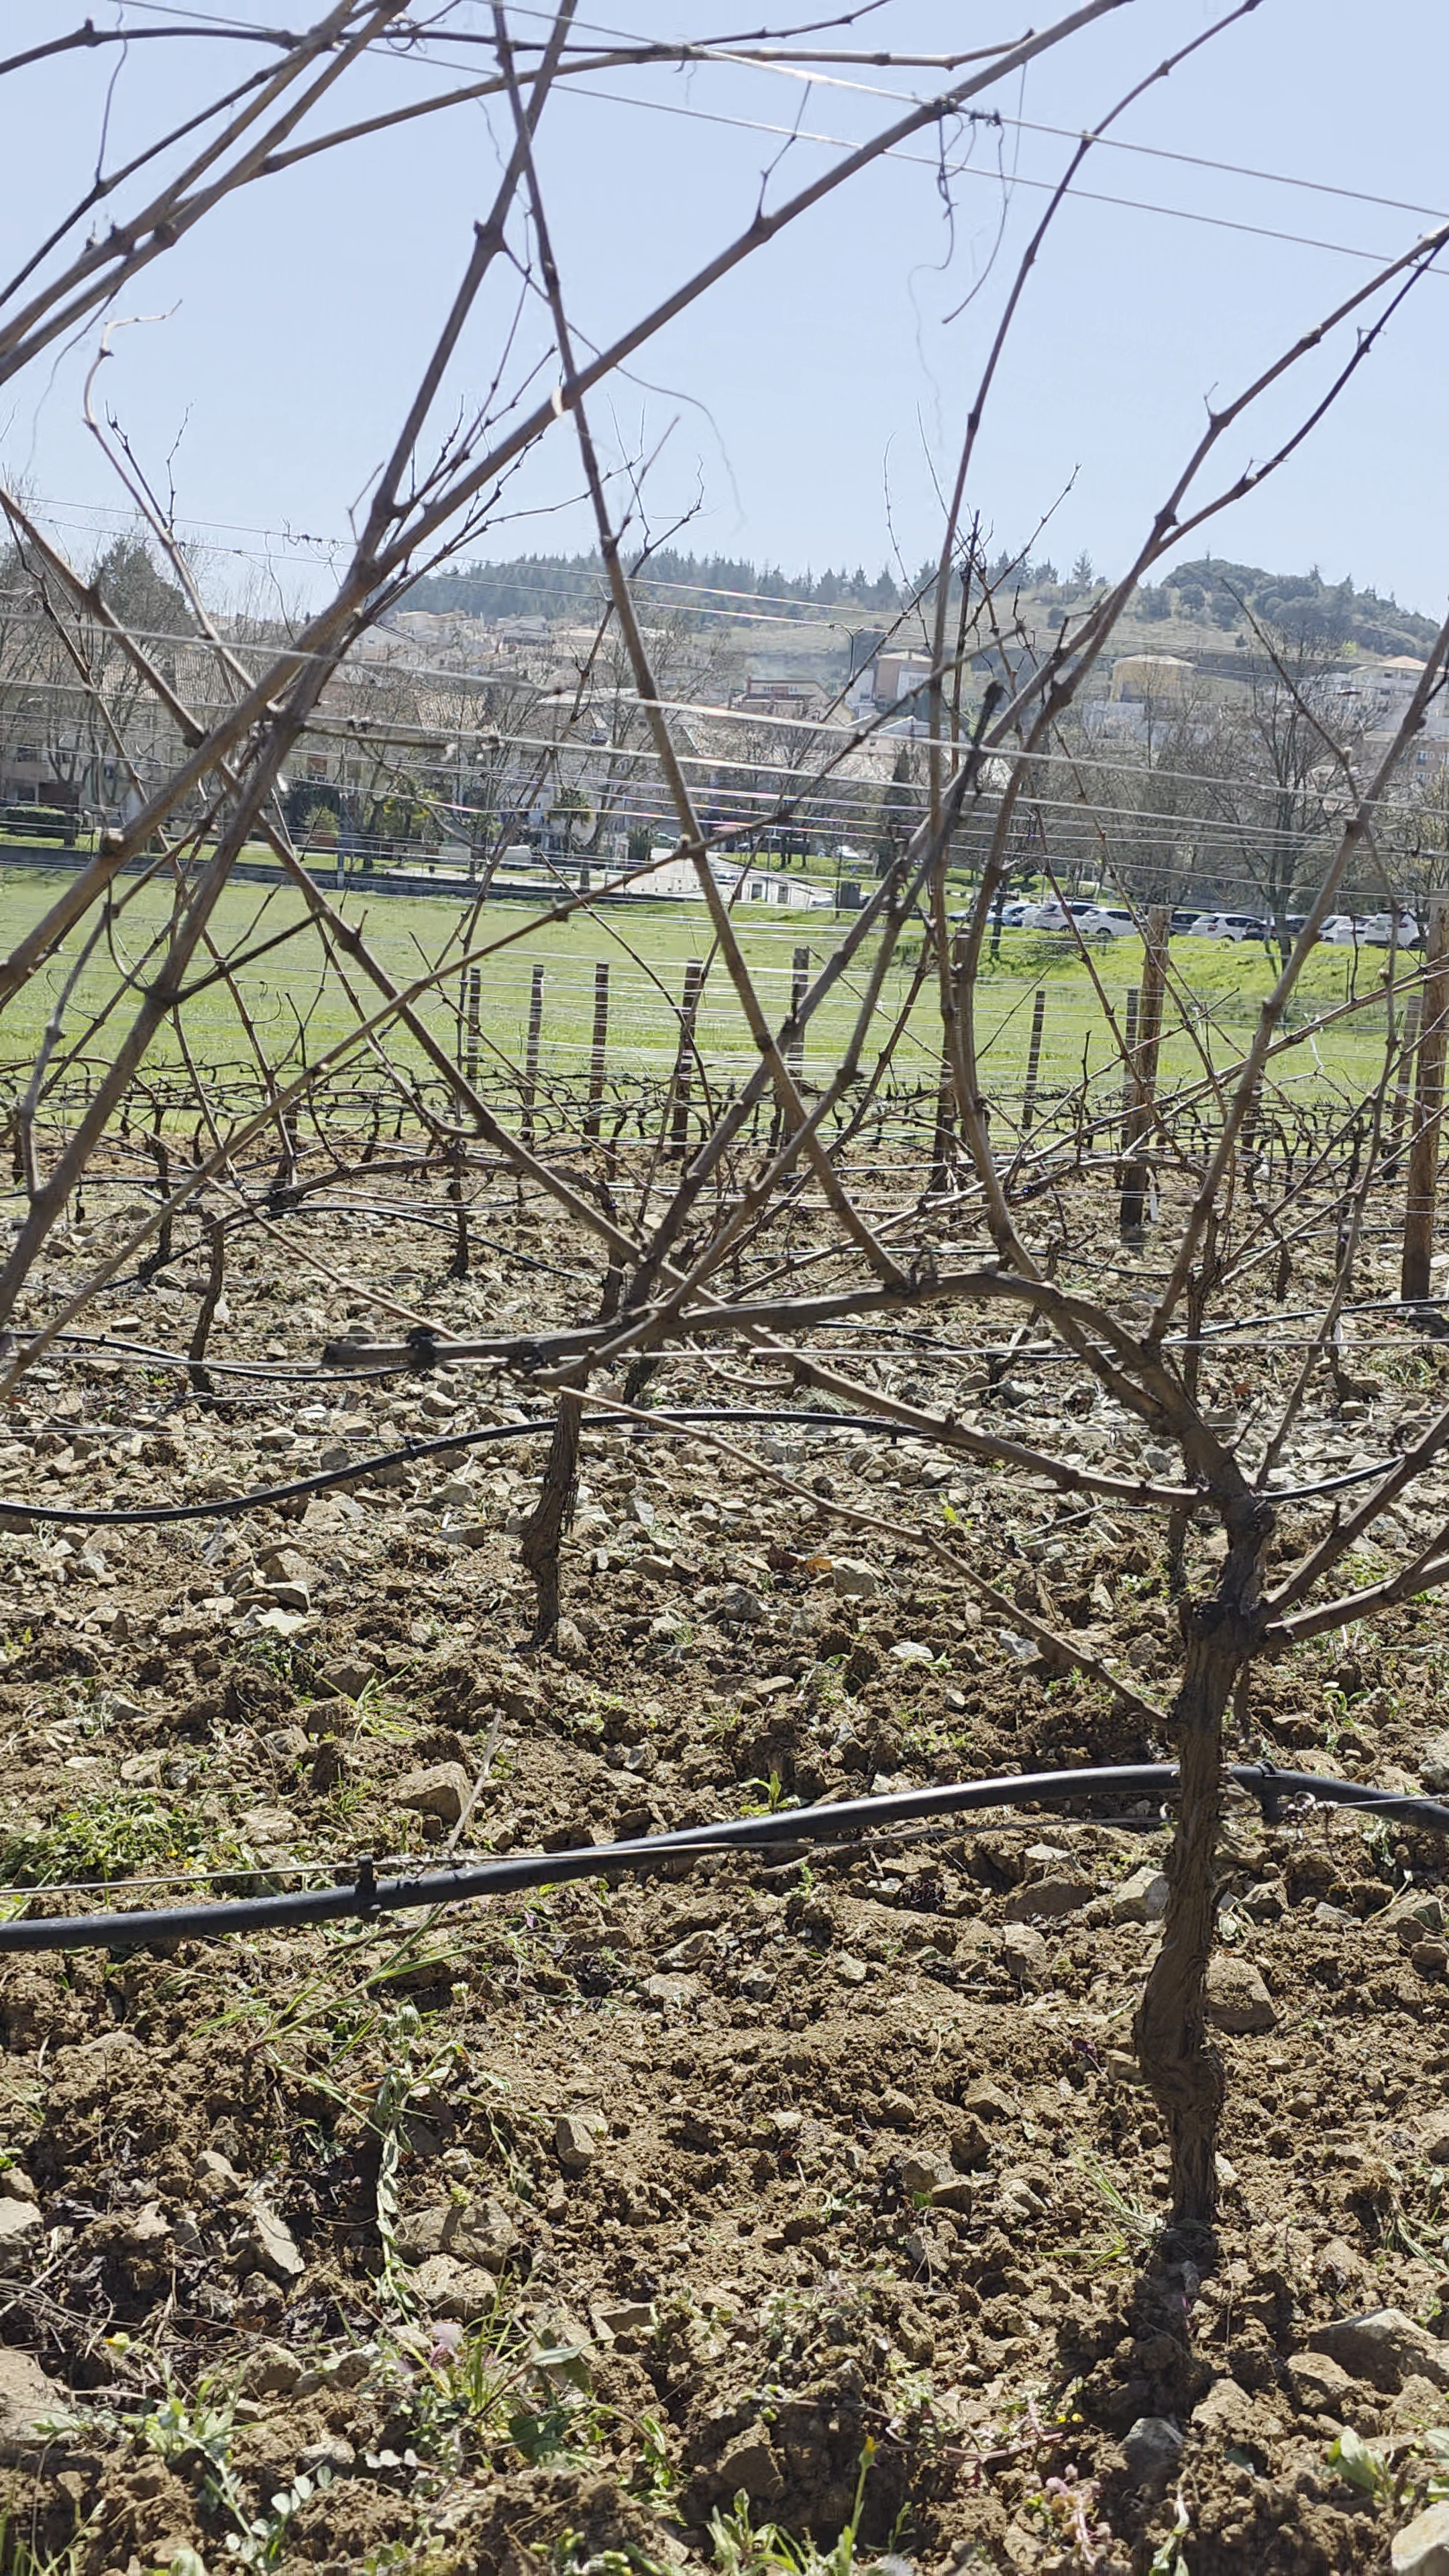
\includegraphics[width=\textwidth]{imagens/videiras_palmela.jpg}
    \caption{Imagem original}
  \end{subfigure}
  \hfill
  \begin{subfigure}[b]{0.47\textwidth}
    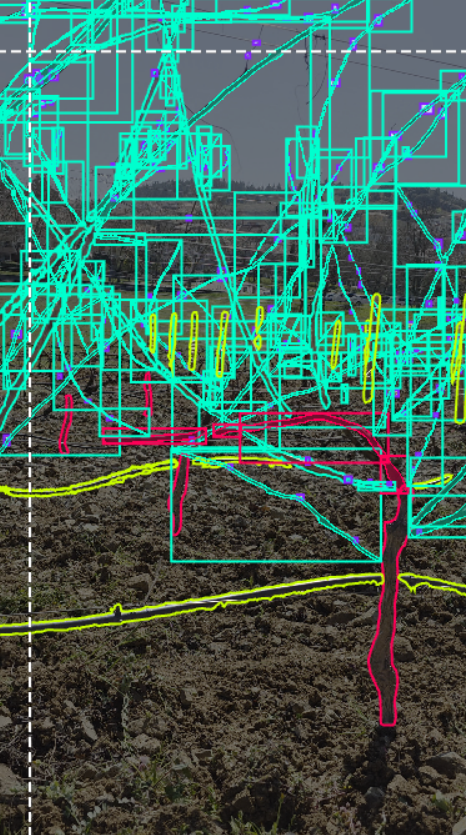
\includegraphics[width=\textwidth]{imagens/videiras_anotadas.png}
    \caption{Com anotações (>300 \textit{bounding boxes})}
  \end{subfigure}

  \vspace{0.5em}
  \caption{Exemplo de imagem anotada das vinhas de Palmela.}
  \label{fig:anotacao}
\end{figure}

As anotações revelam uma densidade de instâncias muito elevada: em média,
cada imagem das vinhas de Palmela contém cerca de \textbf{300 etiquetas}
(\textit{labels}), distribuídas principalmente pelas classes \textit{gomo}
e \textit{sarmento}. A título de exemplo, a imagem representada na
Figura~\ref{fig:anotacao} contém 329 anotações — 161 gomos, 141 sarmentos,
19 objetos e 8 troncos. Esta densidade excede largamente a média de datasets
de deteção de objetos convencionais e constitui um dos principais desafios
técnicos do projeto.

\subsection{Modelos}

Os modelos da família YOLO (\textit{You Only Look Once})~\cite{redmon2016you}
tornaram-se referência para deteção em tempo real, combinando velocidade e
precisão numa única passagem pela rede. O modelo selecionado foi o
\textit{YOLO26 Nano}~\cite{hidayatullah2026yolo26},
desenvolvido pela Ultralytics e lançado em janeiro de 2026 com o lema
\textit{"Built End-to-End. Built for the Edge"}. As principais inovações
relevantes para este trabalho são:

\begin{itemize}[noitemsep]
  \item \textit{End-to-End NMS-free inference}: eliminação da etapa de
    pós-processamento NMS (\textit{Non-Maximum Suppression}), com ganho
    de 43\% na velocidade em modo CPU;
  \item \textit{STAL} (\textit{Small-Target-Aware Label Assignment}):
    garante um mínimo de quatro âncoras para objetos com dimensão inferior
    a 8$\times$8~px, crucial para gomos de pequena dimensão;
  \item \textit{PSABlock} no \textit{neck}: mecanismo de atenção global
    que melhora a representação de características sem custo computacional
    elevado;
  \item \textit{MuSGD}: otimizador híbrido SGD/Muon que melhora a
    convergência em datasets de dimensão reduzida.
\end{itemize}

A Figura~\ref{fig:arch} apresenta o diagrama de arquitetura do YOLO26.

\begin{figure}[H]
  \centering
  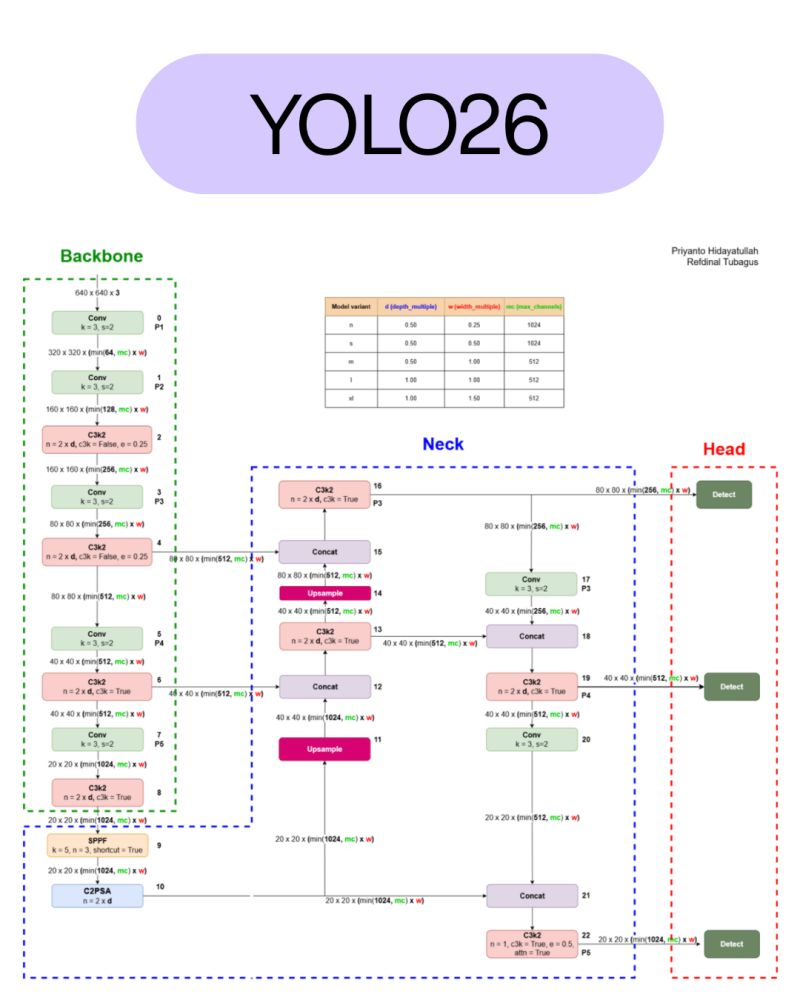
\includegraphics[width=0.95\textwidth]{imagens/YOLOV26_ARCH.jpg}
  \caption{Arquitetura do YOLO26 Nano: Backbone (C3k2 + SPPF com atalho
           residual), Neck (C2PSA com PSABlock) e três cabeças de deteção.
           Fonte:~\cite{hidayatullah2026yolo26}.}
  \label{fig:arch}
\end{figure}

\subsection{Procedimento de Treino}

A plataforma Roboflow~\cite{roboflow2020} tem emergido como ferramenta
de referência para anotação, gestão de versões e treino de modelos em
domínios agrícolas, combinando interface de anotação manual com
funcionalidades de \textit{data augmentation} e treino na nuvem.
O treino foi realizado na plataforma \textit{Roboflow Train} (nuvem),
dispensando infraestrutura local com GPU. A Tabela~\ref{tab:treino} resume
a configuração utilizada em ambos os modelos.

\begin{table}[H]
  \centering
  \caption{Configuração de treino (ambos os modelos)}
  \label{tab:treino}
  \begin{tabular}{ll}
    \toprule
    \textbf{Parâmetro}       & \textbf{Valor} \\
    \midrule
    Plataforma               & Roboflow Train (nuvem) \\
    Modelo base              & YOLO26 Nano (pesos COCO) \\
    Épocas                   & 100 \\
    Tamanho de imagem        & 640$\times$640~px \\
    Divisão treino/val/teste & 70\% / 20\% / 10\% \\
    \bottomrule
  \end{tabular}
\end{table}

%--------------------------------------------------------------------------
% 4. RESULTADOS E DISCUSSÃO
%--------------------------------------------------------------------------
\section{Resultados e Discussão}

\subsection{Modelo 1 — \textit{Segmentation-Vineyard-2}}

O Modelo~1 foi treinado exclusivamente sobre as 300 imagens do
\textit{Segmentation-Vineyard-2}, com as anotações de \textit{gomo}
adicionadas manualmente, perfazendo três classes (\textit{gomo},
\textit{sarmento}, \textit{tronco}). Representa o primeiro treino com
anotações de \textit{sarmento} — versões experimentais anteriores (março
de 2026, apenas \textit{gomos}, $\sim$41 imagens) produziram resultados
insatisfatórios e não são consideradas neste estudo. O Roboflow expandiu
este conjunto para exactamente 775 imagens através de \textit{data augmentation}.
O objetivo deste modelo foi estabelecer uma \textit{baseline} formal sobre
o dataset público, isolando a contribuição das imagens de Palmela nos
modelos subsequentes. A Tabela~\ref{tab:resultados_m1} apresenta as
métricas obtidas no conjunto de validação.

\begin{table}[H]
  \centering
  \caption{Métricas do Modelo 1 — conjunto de validação}
  \label{tab:resultados_m1}
  \begin{tabular}{lc}
    \toprule
    \textbf{Métrica} & \textbf{Valor} \\
    \midrule
    mAP@50           & 49,5\% \\
    Precisão         & 64,2\% \\
    Recall           & 51,3\% \\
    F1               & 57,0\% \\
    \bottomrule
  \end{tabular}
\end{table}

A Figura~\ref{fig:resultado_m1} mostra uma inferência do Modelo~1 com
\textit{confidence threshold} de 12\%.

\begin{figure}[H]
  \centering
  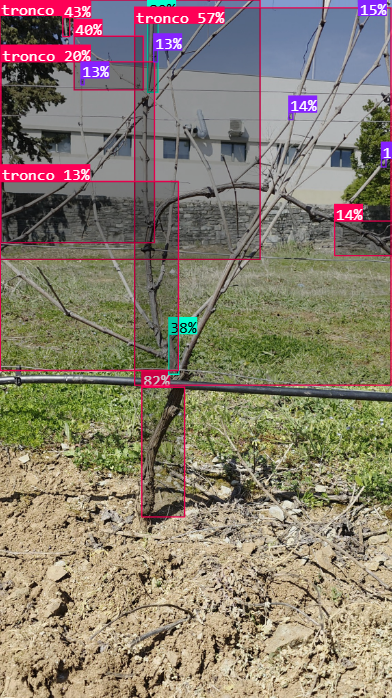
\includegraphics[width=0.60\textwidth]{imagens/modelo1.png}
  \caption{Inferência do Modelo~1 (\textit{threshold} = 12\%). Troncos
           (vermelho), sarmentos (ciano), gomos (roxo). O modelo identifica
           corretamente vários gomos nas posições de inserção nos sarmentos,
           mas classifica incorretamente múltiplos galhos como troncos e
           sub-deteta os sarmentos.}
  \label{fig:resultado_m1}
\end{figure}

A análise qualitativa da inferência revela um comportamento coerente com
um modelo treinado num dataset de domínio único (vinhas espanholas) e
avaliado numa imagem de Palmela:
\begin{itemize}[noitemsep]
  \item \textit{Gomos}: quatro instâncias detetadas com confiança de
    14--15\%, correctamente posicionadas nas inserções dos sarmentos,
    resultado promissor para um primeiro modelo com apenas três classes;
  \item \textit{Sarmentos}: apenas dois detetados (38\% e 82\%), reflectindo
    a diferença visual entre os sarmentos das imagens de treino espanholas
    e os de Palmela;
  \item \textit{Troncos}: múltiplas deteções incorrectas sobre galhos e
    sarmentos, com caixas sobrepostas, indicando que o modelo aprendeu
    a associar estruturas verticais em geral à classe \textit{tronco} em
    vez de distinguir o eixo lenhoso principal.
\end{itemize}

Estes resultados motivaram a introdução da classe \textit{objeto} e a
inclusão de imagens de Palmela nos modelos seguintes, de modo a melhorar
a distinção entre \textit{tronco} e \textit{sarmento} em contexto real.

\subsection{Modelo 2 — SVY-2 + Palmela}

O Modelo~2 incorpora 22 imagens de Palmela ao dataset do Modelo~1,
perfazendo 322 imagens base com quatro classes; o Roboflow gerou 772
imagens para treino através de augmentation. A Tabela~\ref{tab:resultados}
apresenta as métricas obtidas no conjunto de validação.

\begin{table}[H]
  \centering
  \caption{Métricas do Modelo 2 — conjunto de validação}
  \label{tab:resultados}
  \begin{tabular}{lc}
    \toprule
    \textbf{Métrica} & \textbf{Valor} \\
    \midrule
    mAP@50           & 48,8\% \\
    Precisão         & 54,3\% \\
    Recall           & 52,7\% \\
    F1               & 53,5\% \\
    \bottomrule
  \end{tabular}
\end{table}

Um mAP@50 de 48,8\% é um resultado moderado mas coerente com as
características do problema: domínio misto (espanhol + português),
quatro classes com densidades de instâncias muito distintas e uma classe
(\textit{gomo}) completamente nova relativamente ao dataset original. A
precisão (54,3\%) e o recall (52,7\%) equilibrados indicam que o modelo
distribui as dificuldades de forma homogénea entre falsos positivos e
falsos negativos, sem enviesamento sistemático para nenhuma classe.

\subsection{Modelo 3 — Dataset Expandido}

O Modelo~3 representa o estado mais avançado do desenvolvimento, treinado
sobre 938 imagens (geradas por augmentation a partir das imagens base
disponíveis até 17 de junho de 2026). A Tabela~\ref{tab:resultados3} apresenta as
métricas obtidas no conjunto de validação.

\begin{table}[H]
  \centering
  \caption{Métricas do Modelo 3 (V3) — conjunto de validação}
  \label{tab:resultados3}
  \begin{tabular}{lc}
    \toprule
    \textbf{Métrica} & \textbf{Valor} \\
    \midrule
    mAP@50           & 43,7\% \\
    Precisão         & 57,3\% \\
    Recall           & 40,5\% \\
    F1               & 47,4\% \\
    \bottomrule
  \end{tabular}
\end{table}

A Figura~\ref{fig:resultado_v3} mostra uma inferência do Modelo~3 sobre
uma imagem das vinhas de Palmela, com \textit{confidence threshold} de 16\%.

\begin{figure}[H]
  \centering
  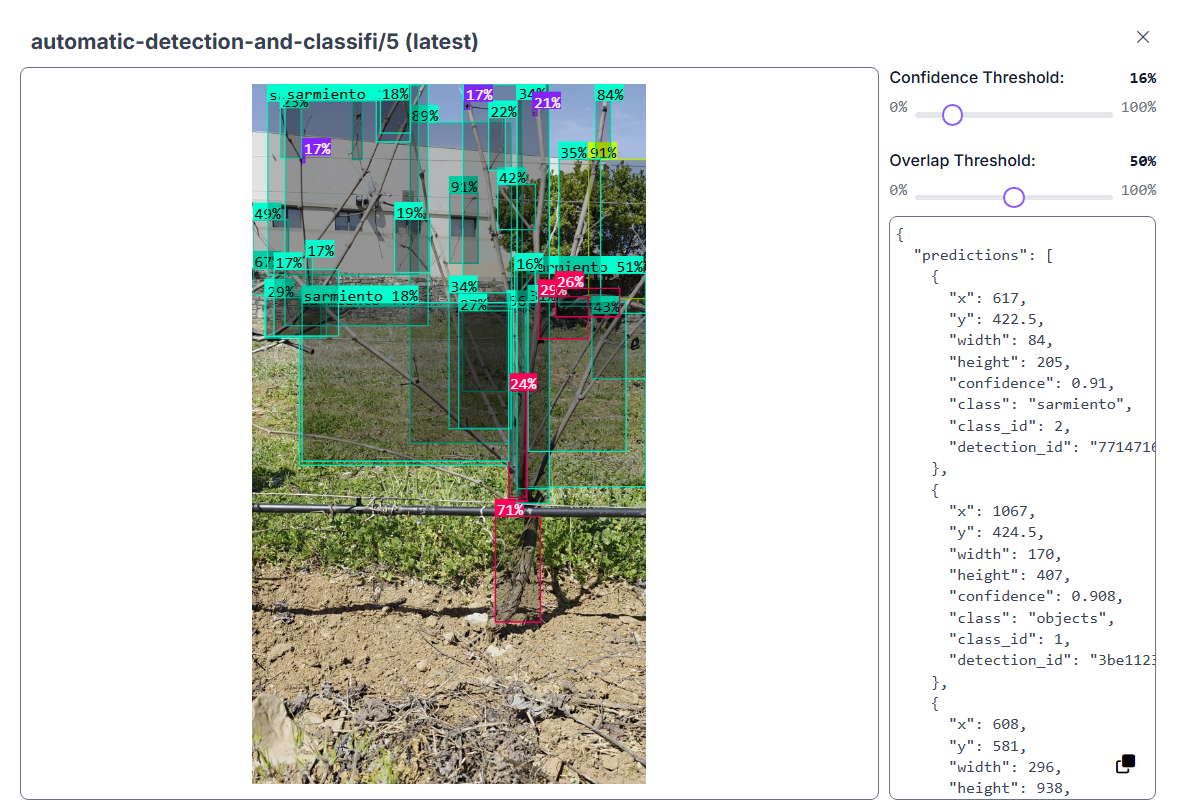
\includegraphics[width=0.82\textwidth]{imagens/resultado_v3.png}
  \caption{Inferência do Modelo~3 sobre imagem das vinhas de Palmela
           (\textit{threshold} = 16\%). Sarmentos (ciano), gomos (roxo),
           objetos (vermelho). Os gomos surgem com confiança baixa (16--26\%),
           enquanto os sarmentos atingem confiança até 91\%.}
  \label{fig:resultado_v3}
\end{figure}

A inferência revela um comportamento que reflete a assimetria de dificuldade
entre classes: os sarmentos são detetados com elevada confiança (até 91\%),
pois são estruturas visualmente distintas e de grande dimensão; os gomos,
em contraste, apenas surgem com \textit{threshold} abaixo de 16\%, o que
indica que o modelo ainda está a calibrar a confiança nesta classe mais difícil,
sendo que os gomos têm dimensão reduzida, apresentam
variabilidade de forma e aparecem com frequências muito distintas entre
imagens, tornando a aprendizagem mais lenta.

\subsection{Discussão Comparativa}

A Tabela~\ref{tab:comparacao} compara as três abordagens desenvolvidas.

\begin{table}[H]
  \centering
  \caption{Comparação entre os modelos desenvolvidos}
  \label{tab:comparacao}
  \begin{tabularx}{\columnwidth}{l X X X}
    \toprule
    \textbf{Aspeto}        & \textbf{Modelo 1} & \textbf{Modelo 2} & \textbf{Modelo 3} \\
    \midrule
    Fontes                 & SVY-2             & SVY-2 + Palmela   & SVY-2 + Palmela \\
    Imagens base           & 300               & 322               & 394 \\
    Imagens (aug.)         & 775               & 772               & 938 \\
    Classes                & 3                 & 4                 & 4 \\
    mAP@50                 & 49,5\%            & 48,8\%            & 43,7\% \\
    Precisão               & 64,2\%            & 54,3\%            & 57,3\% \\
    Recall                 & 51,3\%            & 52,7\%            & 40,5\% \\
    F1                     & 57,0\%            & 53,5\%            & 47,4\% \\
    \bottomrule
  \end{tabularx}
\end{table}

A transição do Modelo~1 para o Modelo~2 mostra que a adição de imagens de
Palmela e de uma quarta classe reduziu ligeiramente o mAP@50 de 49,5\% para
48,8\%, mas manteve métricas globais semelhantes. O Modelo~1 destaca-se pela
Precisão mais elevada (64,2\%), indicando menos falsos positivos, o que é
coerente com um dataset de domínio único e mais homogéneo.
A transição do Modelo~2 para o Modelo~3 evidencia um padrão esperado face
à maior dificuldade do dataset expandido: o mAP@50 desce de 48,8\% para
43,7\%, mas a Precisão sobe de 54,3\% para 57,3\%, indicando menos falsos
positivos. A queda no Recall (de 52,7\% para 40,5\%) reflete a dificuldade
de detetar gomos em imagens de Palmela com maior complexidade visual,
dado que o modelo os deteta, mas a confiança não atinge o limiar convencional de
50\%. A adição contínua de imagens de Palmela é o principal vetor de
melhoria, prevendo-se que alcançar 2000--3000 imagens base resulte num
salto significativo no Recall dos gomos.

%--------------------------------------------------------------------------
% 5. CONCLUSÃO
%--------------------------------------------------------------------------
\section{Conclusão}

Este artigo apresentou o desenvolvimento iterativo de um sistema de deteção
automática de gomos em videiras baseado no YOLO26 Nano, com aplicação a
sistemas robóticos de poda mecanizada. Foram desenvolvidos três modelos
progressivos, de 300 imagens base (775 após \textit{data augmentation})
a 394 imagens base (938 após \textit{data augmentation}), evidenciando uma
metodologia replicável de construção de dataset e treino incremental.

O trabalho demonstrou que: (i) é possível adaptar um dataset público de
sarmentos e troncos para incluir a deteção de gomos através de anotação
manual; (ii) o YOLO26 Nano aprende a estrutura visual de videiras com
datasets de dimensão reduzida, atingindo mAP@50 de 49,5\% no Modelo~1,
48,8\% no Modelo~2 e 43,7\% no Modelo~3 (domínio mais difícil, 4 classes); (iii) a plataforma
Roboflow Train viabiliza o treino de modelos de qualidade sem infraestrutura
local de GPU; (iv) a deteção de gomos em cenas reais é um problema exigente,
pois os gomos surgem com confiança reduzida mesmo no Modelo~3, o que indica
que o volume de dados é ainda insuficiente para calibrar esta classe.

As principais direções de trabalho futuro são: expansão do dataset de
Palmela para 2000--3000 imagens anotadas; avaliação de variantes maiores
do YOLO26 (Small, Medium) à medida que o dataset crescer; integração com
câmeras de profundidade para estimativa 3D dos pontos de corte; e exploração
de YOLO26-Seg para segmentação de instâncias de sarmentos.

%--------------------------------------------------------------------------
% AGRADECIMENTOS
%--------------------------------------------------------------------------
\section*{Agradecimentos}

O autor agradece ao \textit{Research Centre in Digitalization and
Intelligent Robotics} (CeDRI) e ao \textit{Laboratório para a
Sustentabilidade e Tecnologia em Regiões de Montanha} (SusTEC) do
Instituto Politécnico de Bragança pela infraestrutura, orientação e apoio
disponibilizados ao longo deste trabalho, bem como a todos os colegas e
investigadores que contribuíram com sugestões e discussões.

Este trabalho é financiado por fundos nacionais através da FCT, Fundação
para a Ciência e a Tecnologia, I.P., no âmbito dos projetos: CeDRI,
UID/05757/2025 (DOI: \href{https://doi.org/10.54499/UID/05757/2025}{10.54499/UID/05757/2025})
e UID/PRR/05757/2025 (DOI: \href{https://doi.org/10.54499/UID/PRR/05757/2025}{10.54499/UID/PRR/05757/2025});
SusTEC, LA/P/0007/2020 (DOI: \href{https://doi.org/10.54499/LA/P/0007/2020}{10.54499/LA/P/0007/2020}).

%--------------------------------------------------------------------------
% REFERÊNCIAS
%--------------------------------------------------------------------------
\printbibliography[title={Referências}]

%==========================================================================
\end{document}
%==========================================================================
